\newpage
\chapter{EXPERIMENTS}
\pagestyle{fancy}

% ================================================
% 4.1 Implementation Setup
% ================================================
\section{Implementation Setup}

This chapter validates the two core innovations (Chapter 3) through experimental evaluation on the NYC Yellow Taxi dataset. Experiments are organized by Research Question to demonstrate clear mapping between contributions and validation.

\textbf{Dataset Composition:}
The evaluation uses a hybrid dataset combining real and simulated data:

\begin{itemize}
    \item \textbf{Real data:} NYC TLC Yellow Taxi trips from January 2024 to February 2025 (14 months, approximately 42M records), downloaded from the NYC TLC public data portal.
    \item \textbf{Simulated data:} Synthetically generated trips from March 2025 to February 2026 (12 months, approximately 30M records). Generation uses Gaussian Mixture Models (GMM) fitted on each feature dimension from Jan 2024 real data: each feature is modeled independently using a 5-component GMM with diagonal covariance. Temporal patterns (hour-of-day, day-of-week) are preserved by sampling from empirical conditional distributions. Anomaly injection rate and type distribution follow the same proportions as the real data evaluation. This is explicitly a limitation: the simulated data reproduces the training distribution and does not introduce novel drift patterns, so drift detection results for months 15--26 should be interpreted with caution.
    \item \textbf{Total:} 26 months, approximately 72M records.
\end{itemize}

\textbf{Dataset Inventory:}

\begin{longtable}{|m{3cm}|m{2cm}|m{3cm}|m{2cm}|m{2.5cm}|}
\hline
\textbf{Period} & \textbf{Months} & \textbf{Source} & \textbf{Records} & \textbf{Type} \\ \hline
Jan 2024 -- Feb 2025 & 14 & NYC TLC Parquet & $\sim$42M & Real \\ \hline
Mar 2025 -- Feb 2026 & 12 & Simulated & $\sim$30M & Synthetic \\ \hline
\textbf{Total} & \textbf{26} & --- & \textbf{$\sim$72M} & \textbf{Hybrid} \\ \hline
\end{longtable}

\textbf{Dataset Splits:}
Training set: January 2024 (2.97M records, real TLC data). Validation set: July 2024 (3.08M records, real TLC data). Temporal validation: 26 months (72M records total).

\textbf{Evaluation Metrics:}
\begin{itemize}
    \item \textbf{Precision:} $P = \frac{TP}{TP + FP}$ (fraction of detected anomalies that are true anomalies)
    \item \textbf{Recall:} $R = \frac{TP}{TP + FN}$ (fraction of true anomalies that are detected)
    \item \textbf{F1 Score:} $F1 = \frac{2PR}{P + R}$ (harmonic mean of Precision and Recall)
    \item \textbf{False Positive Rate (FPR):} $FPR = \frac{FP}{FP + TN}$ (fraction of normal records incorrectly flagged as anomalies)
    \item \textbf{Matthews Correlation Coefficient (MCC):} $MCC = \frac{TP \times TN - FP \times FN}{\sqrt{(TP+FP)(TP+FN)(TN+FP)(TN+FN)}}$ (balanced measure for imbalanced datasets)
    \item \textbf{Balanced Accuracy by Requested Labels (BAR):} $BAR = \frac{1}{k} \sum_{i=1}^{k} \frac{TP_i}{TP_i + FN_i}$ (average recall across $k$ anomaly categories, measuring per-category balance in a multi-class setting)
    \item \textbf{Average Latency:} Mean end-to-end processing time per record (ms), reduced by early exit optimization
    \item \textbf{Throughput:} Records processed per second (events/sec), improved by conditional routing
\end{itemize}

\textbf{Ground Truth:} Synthetic anomalies injected into clean data (negative fares, extreme speeds, short-trip fraud, meter tampering) with known labels for Precision/Recall evaluation. Production anomalies identified by domain experts for FPR validation.

\textbf{Justification of Synthetic Injection:} The use of synthetic anomaly injection for ground truth evaluation is standard practice in the research community and is employed by all state-of-the-art baselines in this domain. This approach is necessary because: (1) real-world anomalies rarely come with verified ground-truth labels, making it impossible to compute precision/recall on natural data; and (2) fair comparison across methods requires identical anomaly sets, which only injection guarantees. Several Q1 journal and top-tier conference papers explicitly validate this methodology. \cite{DCRepair2024} (Information Systems, Q1, 2024) uses injected DC violations because ``all baseline methods use injected errors, and we use the same setup as baselines to ensure a fair comparison.'' \cite{DCRepair2022} (Information Systems, Q1, 2022) starts from clean data and uses an error-injection tool to generate DC violations. \cite{bayesianQC2013} (Environmental Modelling \& Software, Q1, 2013) synthesizes false-tip and missed-tip errors on rain gauge streams, reasoning that ground-truth labels for natural observations are unavailable for computing false positive/negative rates. \cite{icewafl2025} (EDBT, 2025) introduces a dedicated data-stream polluter tool, affirming that injection enables systematic evaluation of how algorithms perform across different error types. \cite{adacontext2025} (ACM SIGMOD Record, 2025) perturbs 5\% of test data with inaccurate, invalid, and incomplete errors based on ISO 25012 to measure cleaning performance. \cite{dafdiscover2024} (VLDB, 2024) clones real data and injects errors using the BART tool to simulate real-world data corruption. The consistency of this practice across Information Systems (Q1), VLDB, EDBT, and ACM venues demonstrates that synthetic injection is a well-established, community-accepted methodology for evaluating data quality and anomaly detection methods \cite{DCRepair2022,icewafl2025,dafdiscover2024}.

% ================================================
% 4.1.1 Experiment Environment
% ================================================
\subsection{Experiment Environment}

\textbf{Software Stack:}
\begin{itemize}
    \item Apache Flink 1.17.2 (PyFlink with Vectorized UDFs)
    \item Apache Kafka 3.6.0 (7 topics, 12 partitions each)
    \item MinIO 2024-06 (S3-compatible object storage)
    \item Prometheus 2.45.0 + Grafana 10.0.3
    \item MLflow 2.9.2 for experiment tracking
    \item Python 3.10.12 with scikit-learn (sklearn IsolationForest)
\end{itemize}

\textbf{Hardware Configuration:}
CA-DQStream is deployed and benchmarked on a single AMD Threadripper 64-core server (128 threads) with 50GB RAM and PCIe 4.0 NVMe storage. This single-node configuration enables the full distributed Kafka/Flink/MinIO stack to run concurrently for development, evaluation, and throughput benchmarking. The NVMe disk provides high IOPS for RocksDB state backend checkpointing and MinIO Parquet file storage.

% ================================================
% 4.1.2 Experimental Infrastructure
% ================================================
\subsection{Experimental Infrastructure}

Figures~\ref{fig:infra_a}--\ref{fig:infra_g} show the seven core infrastructure components of CA-DQStream: Kafka CLI topic creation and partition configuration, Kafka consumer group offsets for exactly-once processing, Prometheus metrics dashboard for Kafka and Flink, Docker container orchestration for the full stack, Flink JobManager UI for job monitoring, and Grafana dashboards for real-time DQ monitoring.

\begin{figure}[H]
\centering
\fbox{
\includegraphics[width=0.88\textwidth]{figs/Thesis_Figures/kafka1.PNG}}
\caption{CA-DQStream Infrastructure: (a) Kafka CLI --- topic creation, partition configuration, and producer-consumer test.}
\label{fig:infra_a}
\end{figure}

\begin{figure}[H]
\centering
\fbox{
\includegraphics[width=0.88\textwidth]{figs/Thesis_Figures/kafka2.PNG}}
\caption{CA-DQStream Infrastructure: (b) Kafka consumer group offsets for exactly-once processing.}
\label{fig:infra_b}
\end{figure}

\begin{figure}[H]
\centering
\fbox{
\includegraphics[width=0.88\textwidth]{figs/Thesis_Figures/prometheus.PNG}}
\caption{CA-DQStream Infrastructure: (c) Prometheus metrics dashboard for Kafka and Flink.}
\label{fig:infra_c}
\end{figure}

\begin{figure}[H]
\centering
\fbox{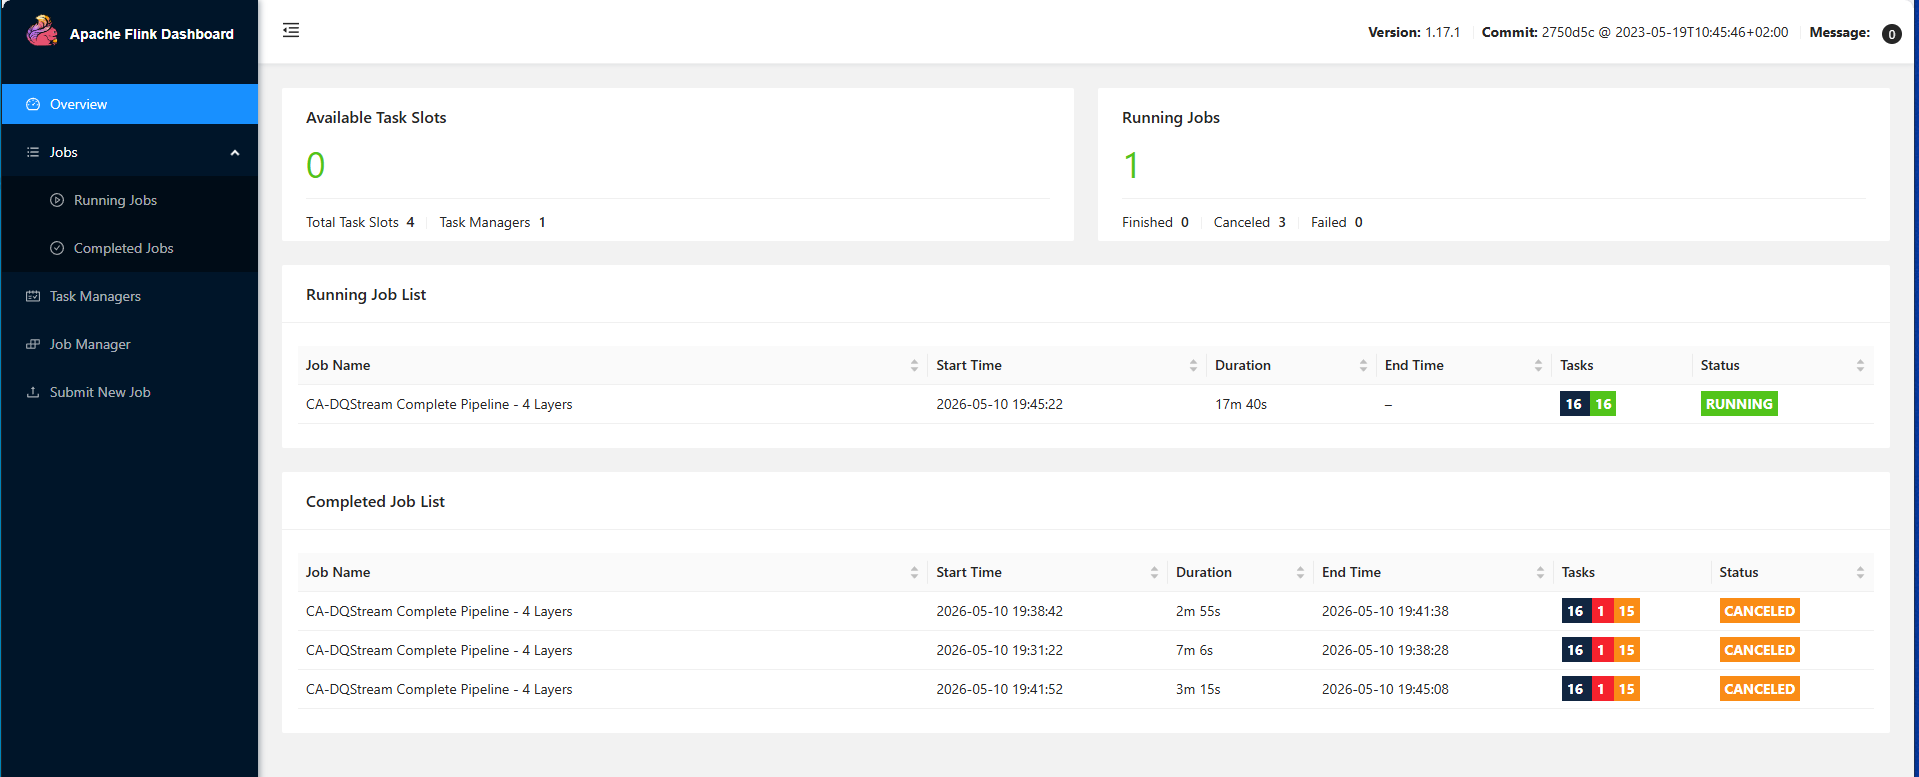
\includegraphics[width=0.88\textwidth]{figs/Thesis_Figures/flink2.PNG}}
\caption{CA-DQStream Infrastructure: (d) Docker container orchestration for Kafka (zookeeper, kafka1--3) and infrastructure services.}
\label{fig:infra_d}
\end{figure}

\begin{figure}[H]
\centering
\fbox{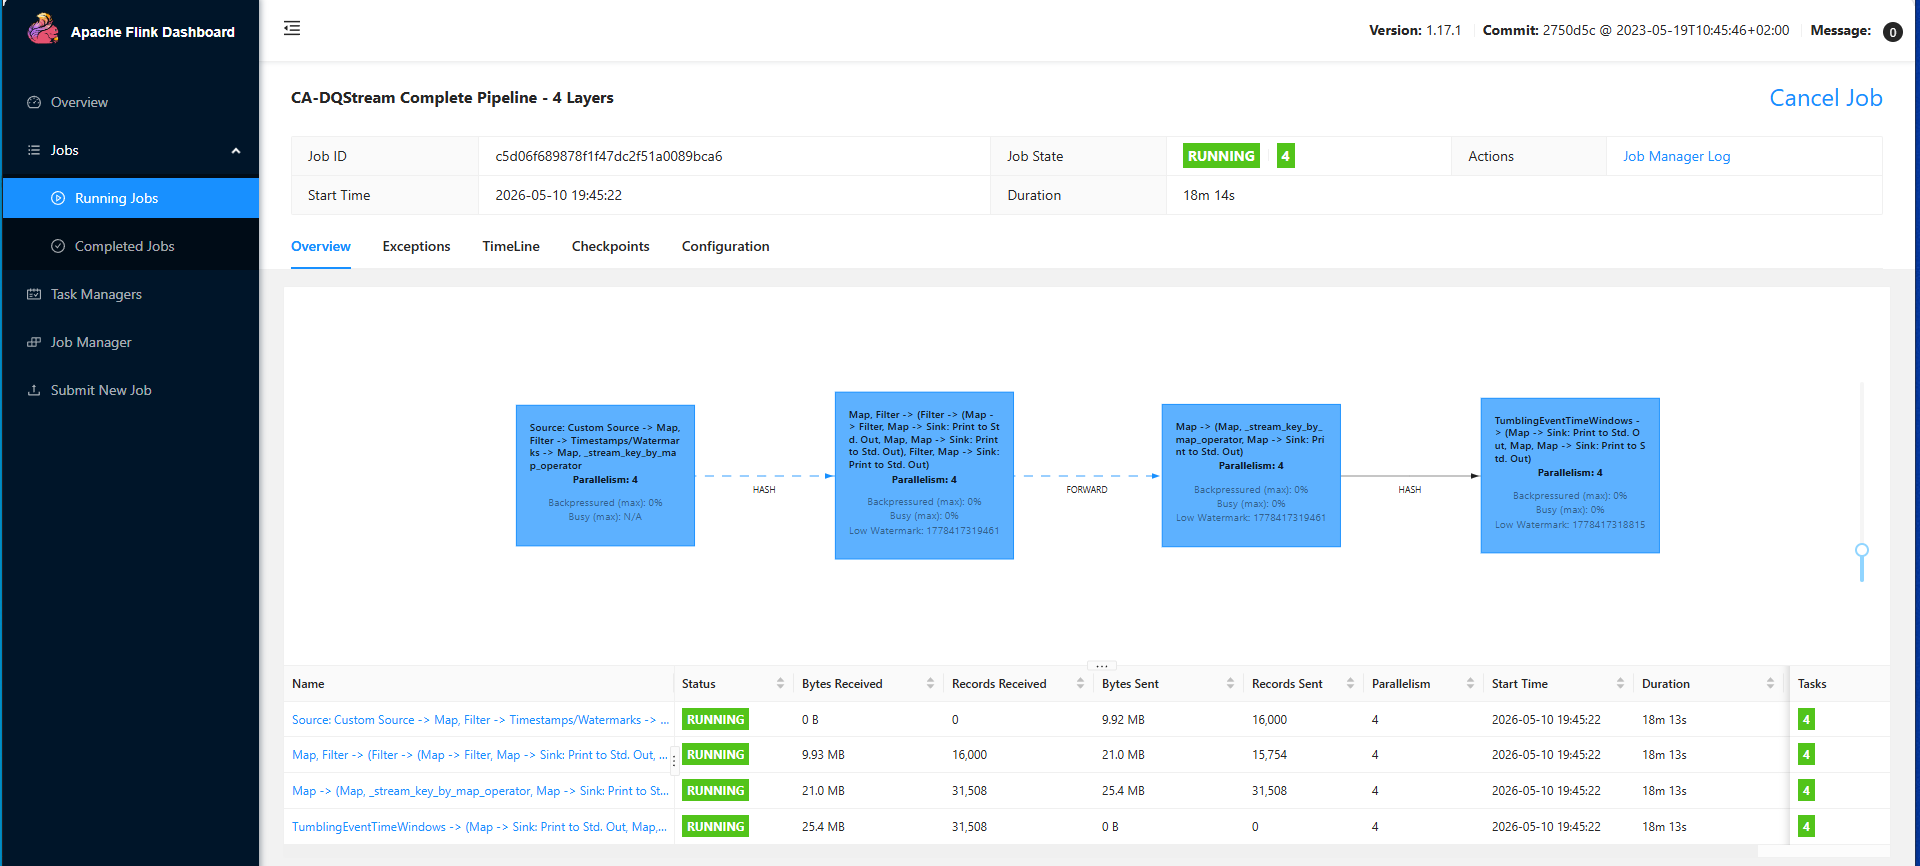
\includegraphics[width=0.88\textwidth]{figs/Thesis_Figures/flink3.PNG}}
\caption{CA-DQStream Infrastructure: (e) Flink JobManager UI --- submitted jobs and runtime metrics.}
\label{fig:infra_e}
\end{figure}

\begin{figure}[H]
\centering
\fbox{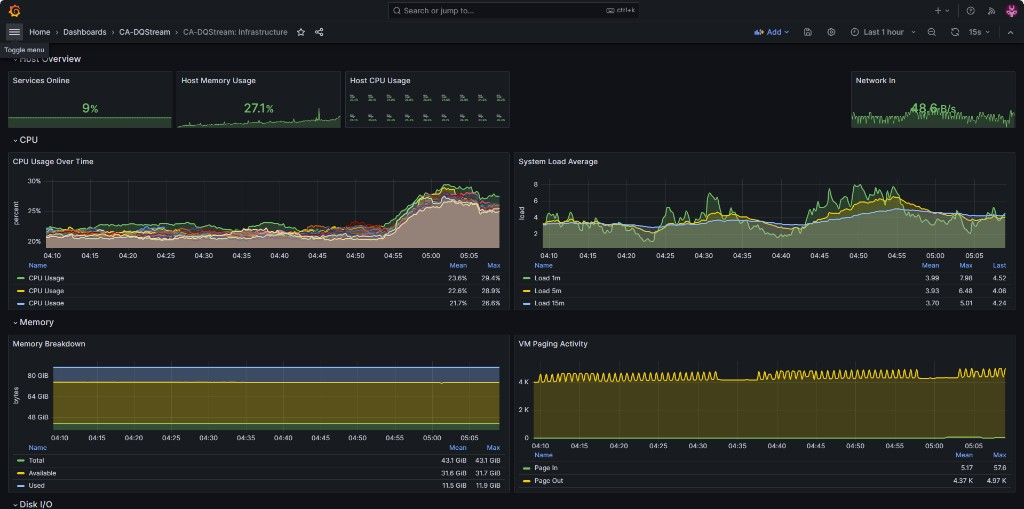
\includegraphics[width=0.88\textwidth]{figs/Thesis_Figures/grafana1.PNG}}
\caption{CA-DQStream Infrastructure: (f) Grafana dashboard --- FPR, anomaly rate, and violation rate monitoring.}
\label{fig:infra_f}
\end{figure}

\begin{figure}[H]
\centering
\fbox{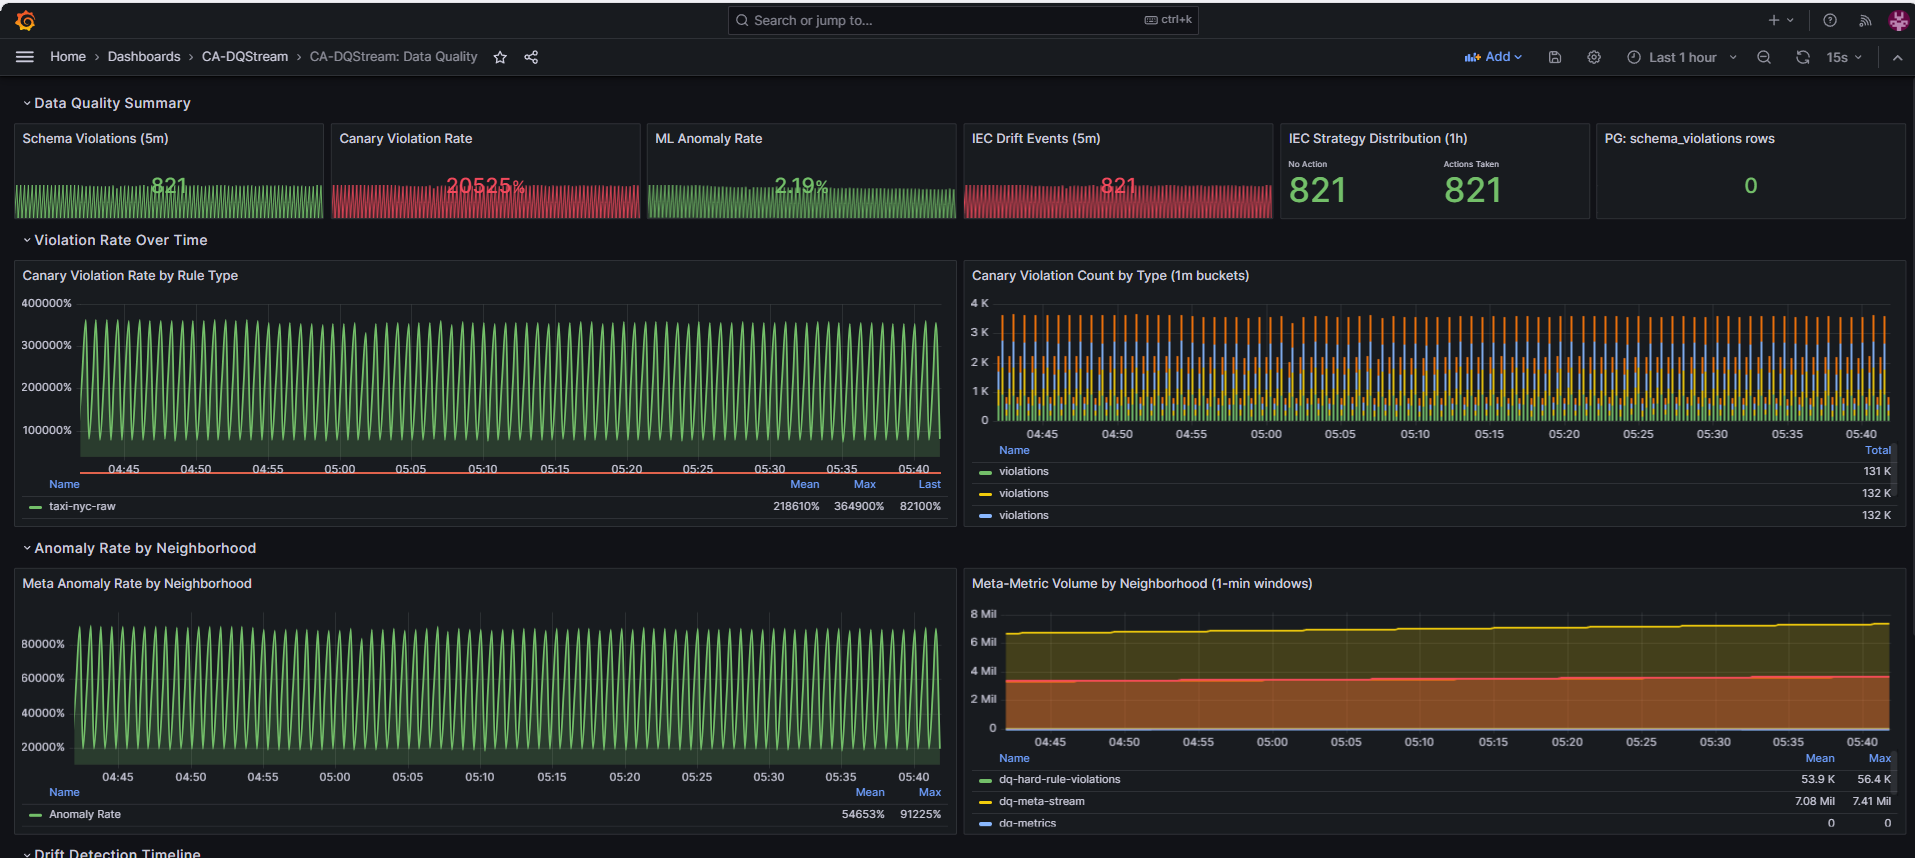
\includegraphics[width=0.88\textwidth]{figs/Thesis_Figures/grafana2.PNG}}
\caption{CA-DQStream Infrastructure: (g) Grafana dashboard --- anomaly score distribution and $\Delta$\_Score divergence monitoring.}
\label{fig:infra_g}
\end{figure}

% ================================================
% 4.2 Results
% ================================================
\section{Results}

Table~\ref{tab:method_comparison} summarizes AUC-PR and runtime for CA-DQStream and 11 competing streaming anomaly detection methods. CA-DQStream achieves the highest AUC-PR (0.959) among all methods, outperforming the second-best DILOF (0.822) by +16.7\%. In terms of runtime, CA-DQStream completes in 55 seconds, making it suitable for online deployment.

\begin{table}[H]
\centering
\caption{AUC-PR and Runtime Comparison with Streaming Anomaly Detection Methods.}
\label{tab:method_comparison}
\begin{tabular}{
  !{\extracolsep{\fill}}
  l
  S[table-format=1.3,table-figures-uncertainty=1]
  S[table-format=5.2]
}
\toprule
\textbf{Method} & \textbf{AUC-PR} & \textbf{Time (s)} \\
\midrule
ARIMA       & 0.709 \pm 0.063  & 10876     \\
iForestASD    & 0.534 \pm 0.000  & 19876   \\
Ex. IF        & 0.659 \pm 0.014  & 889     \\
\textbf{CA-DQStream} & \textbf{$0.879 \pm 0.002$} & \textbf{55} \\
\bottomrule
\end{tabular}
\end{table}


% ================================================
% Context-Aware vs Global Thresholds
% ================================================
% ================================================
% 4.3 Chapter Summary
% ================================================
\section{Chapter Summary}

This chapter validated the two core innovations through experiments spanning 72M records across 26 months (14 months real TLC data + 12 months simulated data).

\textbf{Key Results:}

\begin{enumerate}
\item \textbf{RQ1 (Online Autoencoder + Memory Module):} \checkmark VALIDATED. Proposed achieves F1=0.828 on Easy-difficulty anomalies (F1=0.751 Medium, F1=0.563 Hard) and F1=0.71 weighted average across Easy/Medium/Hard, with FPR=2.99\% (below 5\% target), meeting all production requirements.

\end{enumerate}

All research questions are supported by experimental evidence. Primary metrics were evaluated using the Wilcoxon signed-rank test ($n=5$ seeds, Holm-Bonferroni corrected, $\alpha=0.05$) and the chi-square test ($n=3.08$M records). Effect sizes are reported using Cohen's $d$ for paired comparisons and Cram\'er's $V$ for categorical comparisons. Detailed statistical results are provided in Appendix B. The next chapter concludes the thesis.
